\documentclass{beamer}

\usepackage{pgfplots}
\pgfplotsset{compat=1.17}

\mode<presentation>
{
    \usetheme{Warsaw}
}

\title{CycleMLP}
\subtitle{A MLP-like Architecture for Dense Prediction}
\author{Marco Benelli}
\institute{University of Florence}
\date{February 14, 2022}

\DeclareMathOperator{\layernorm}{LayerNorm}

\begin{document}

\begin{frame}
    \titlepage
\end{frame}

\begin{frame}{Outline}
    \tableofcontents
\end{frame}

\section{Introduction}

\begin{frame}{Paradigm Shifts}
    Recent paradigm shifts:
    \begin{description}
        \item[2012] AlexNet
        \item[2020] ViT
        \item[2021] MLP-Mixer
    \end{description}
\end{frame}

\begin{frame}{MLP-Mixer}
    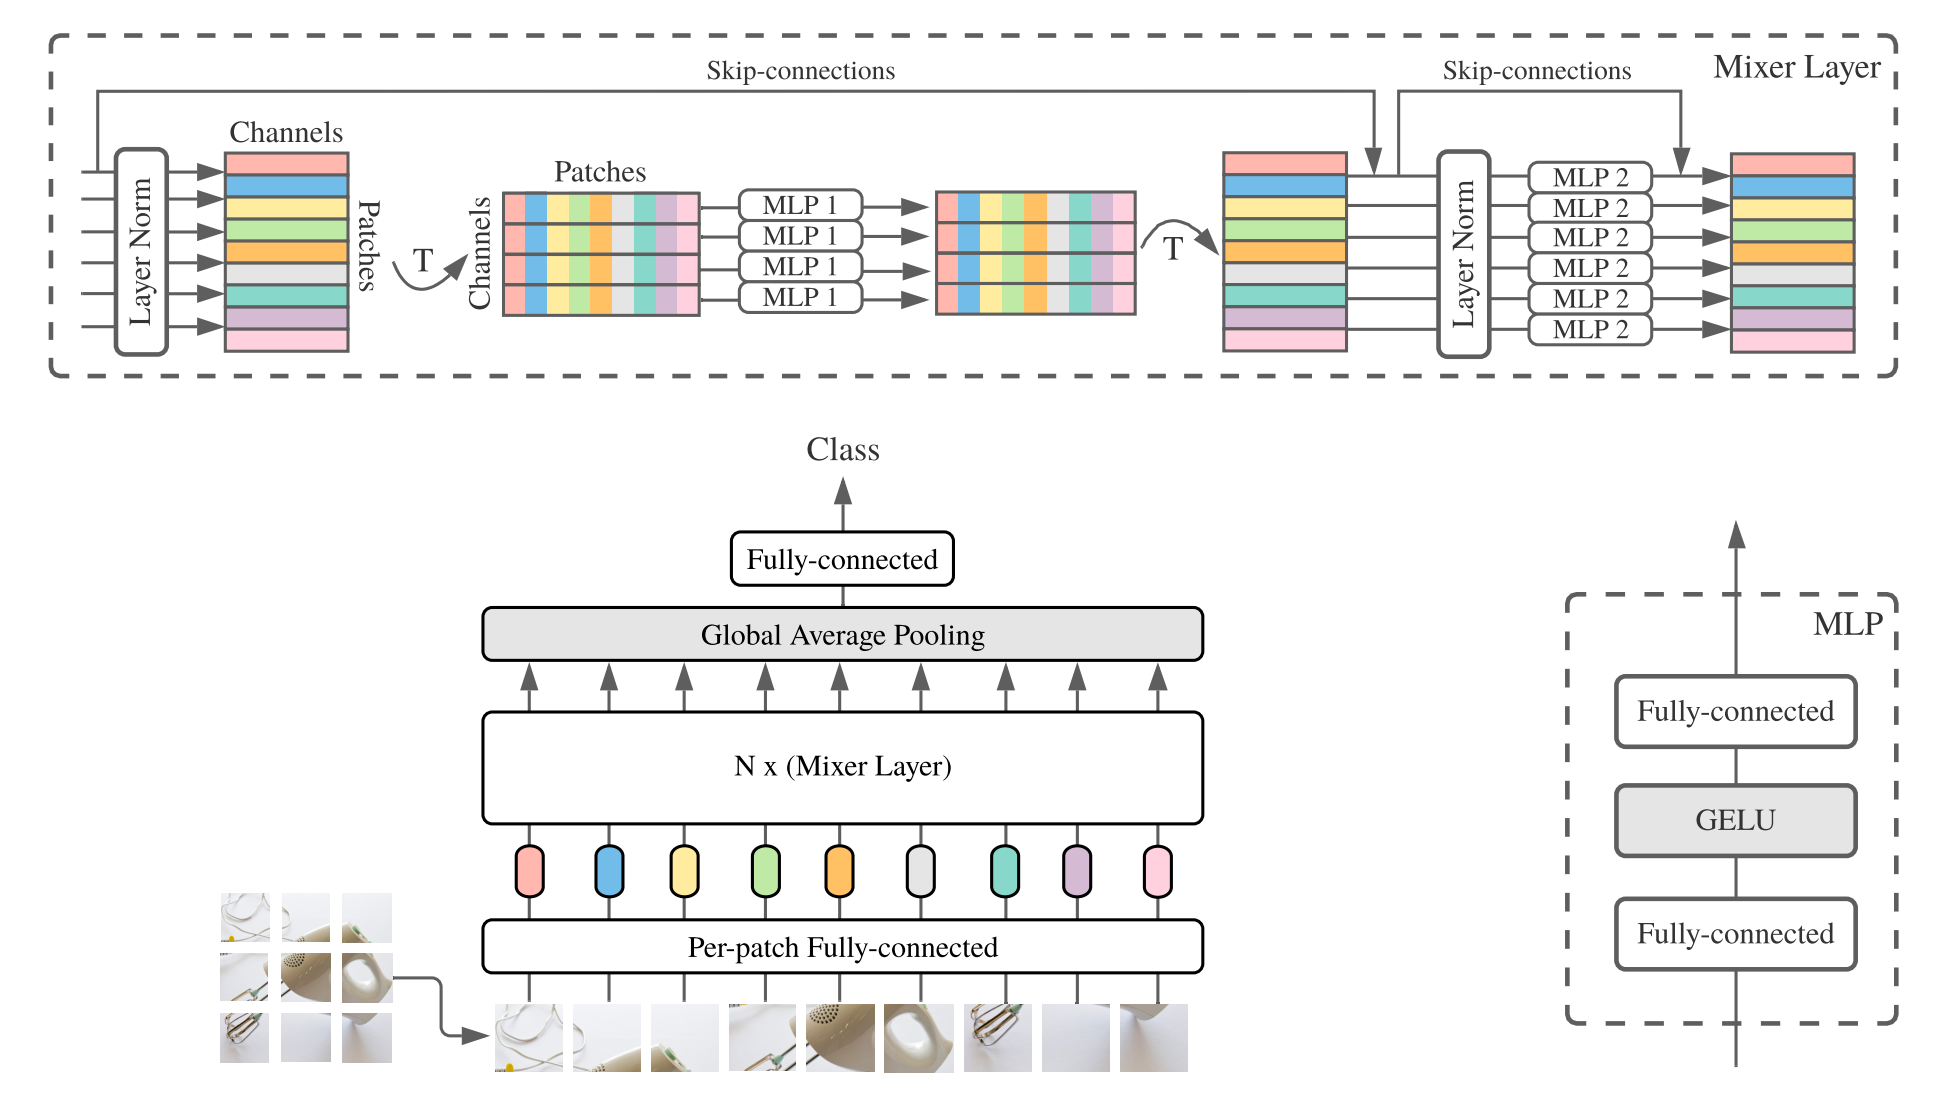
\includegraphics[width=\textwidth]{figures/mixer_figure.png}
\end{frame}

\begin{frame}{Mixer Layer}
    $$\mathbf{U}_{*,i} = \mathbf{X}_{*,i} + \mathbf{W}_2 \sigma(\mathbf{W}_1 \layernorm(\mathbf{X})_{*,i}), \quad \text{for } i = 1 \dots C$$
    $$\mathbf{Y}_{j,*} = \mathbf{U}_{j,*} + \mathbf{W}_4 \sigma(\mathbf{W}_3 \layernorm(\mathbf{U})_{j,*}), \quad \text{for } j = 1 \dots S$$
\end{frame}

\begin{frame}{Challenges}
    MLP-like models are facing these challenges:
    \begin{itemize}
        \item non-hierarchical architectures
        \item flexible input scales
        \item quadratic costs
    \end{itemize}
\end{frame}

\section{Method}

\begin{frame}{MLP-Mixer v. CycleMLP}
    \centering
    \parbox{.4\textwidth}{\centering 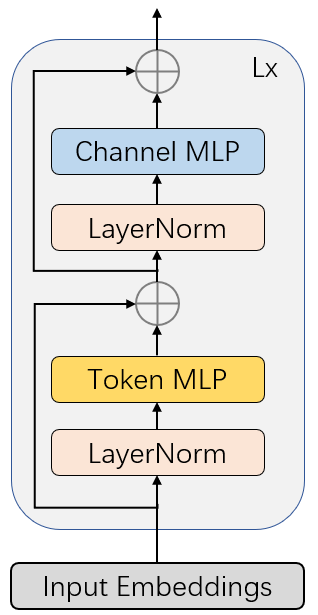
\includegraphics[height=.8\textheight]{figures/mlp_mixer.png}}
    \parbox{.4\textwidth}{\centering 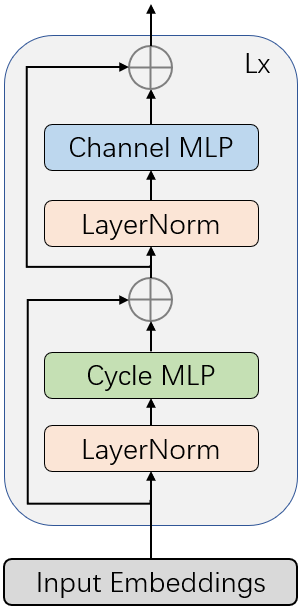
\includegraphics[height=.8\textheight]{figures/cycle_mlp.png}}
\end{frame}

\subsection{Cycle Fully-Connected Layer}

\begin{frame}{Cycle FC}
    \centering
    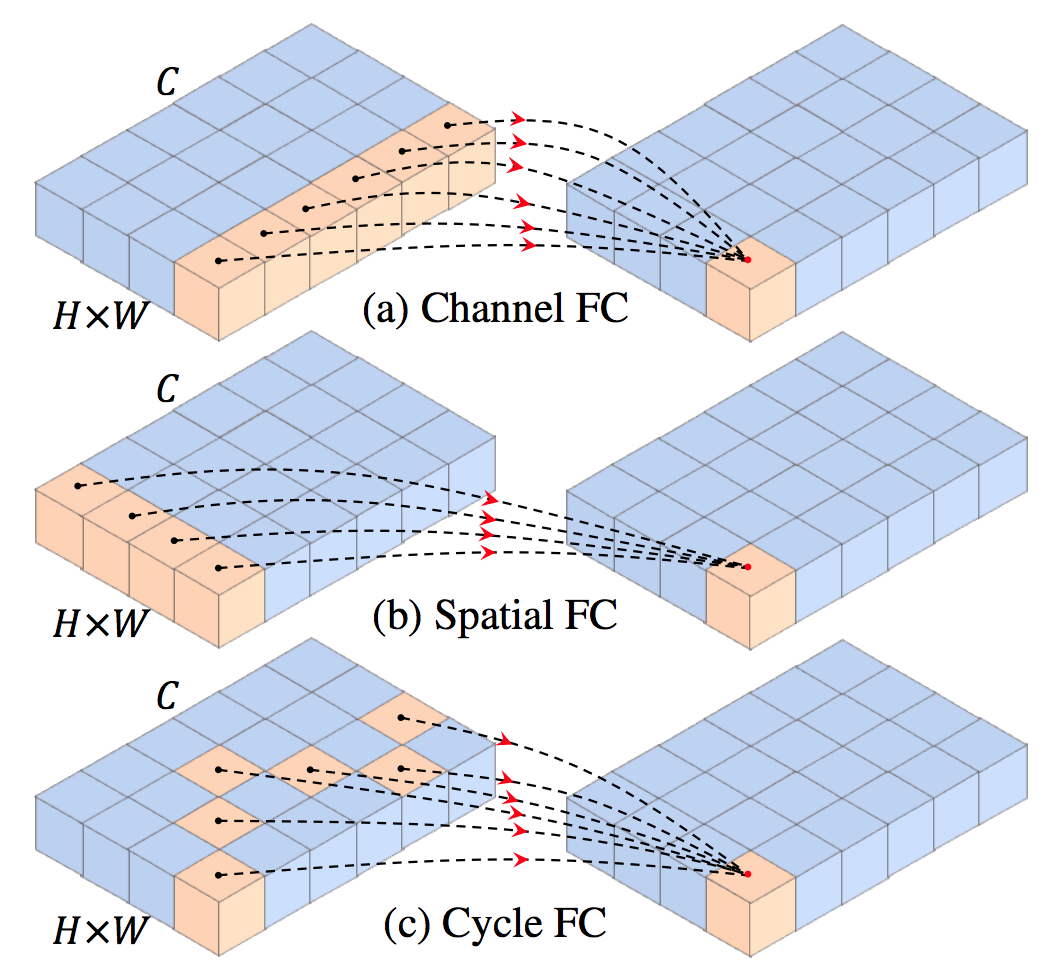
\includegraphics[height=.8\textheight]{figures/teaser.png}
    % \parbox{.4\textwidth}{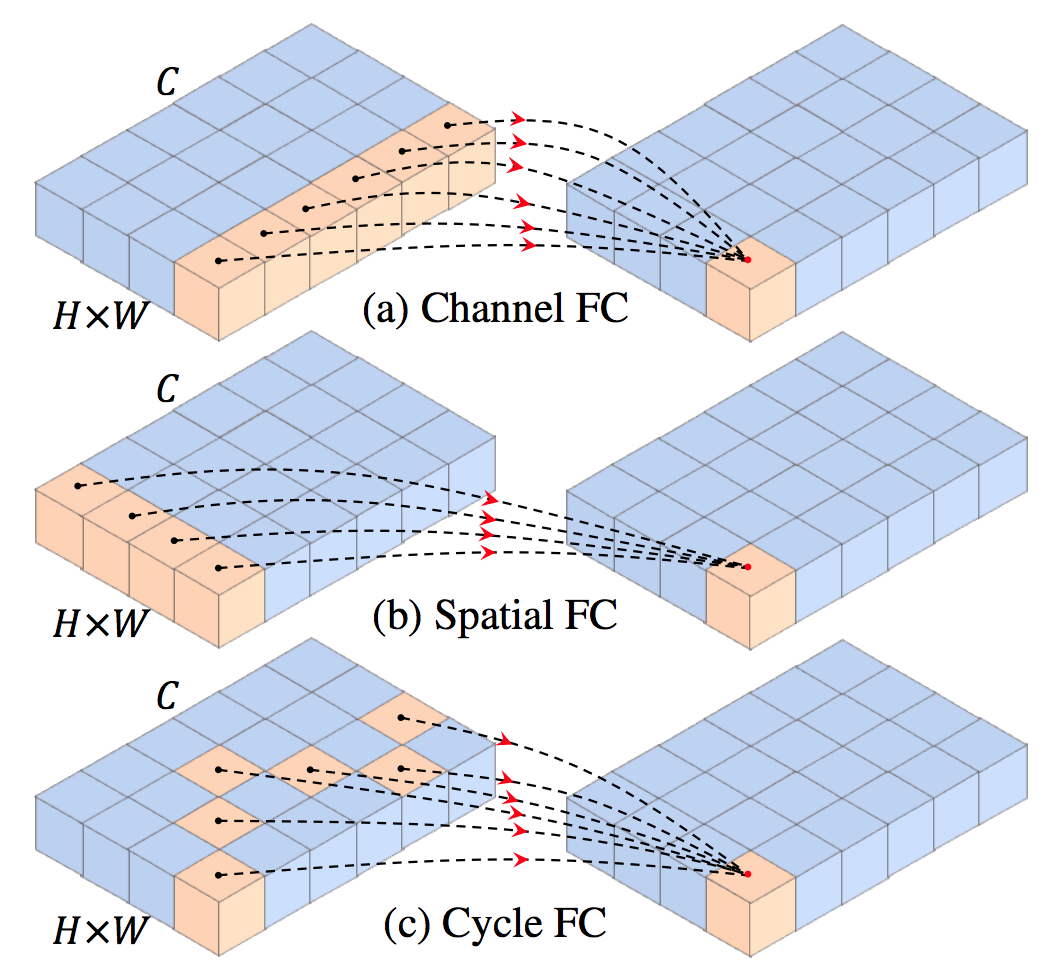
\includegraphics[width=.4\textwidth]{figures/teaser.png}}
    % \parbox{.4\textwidth}{\begin{tabular}{c c c}
    %     \hline
    %     FC & $\mathcal{O}(HW)$ & \begin{tabular}{c}Scale \\ Variable\end{tabular} \\
    %     \hline
    %     Channel & $HW$ & Yes \\
    %     \hline
    %     Spatial & $H^2W^2$ & No \\
    %     \hline
    %     Cycle & $HW$ & Yes \\
    %     \hline
    % \end{tabular}}
\end{frame}

\subsection{Overall Architecture}

\section{Experiments}

\begin{frame}{Experimental Setup}
    \begin{itemize}
        \item optimizer AdamW
        \item $\lambda = 5 \times 10^{-2}$
        \item cosine annealing learning rate schedule
        \item $\eta_{\text{max}} = 1 \times 10^{-3}$
        \item $T_\text{max} = 100$
        \item $\text{batch size} = 256$
    \end{itemize}
\end{frame}

\begin{frame}{Experiments}
    \centering
    \begin{tabular}{c c c c}
        \hline
        Model & STL10 & CIFAR10 & ImageNet-1K \\
        \hline
        ResNet & 64.9\% & 77.1\% \\
        % RegNet & 51.5\% & 60.6\% \\
        ViT & 44.4\% \\
        MLP-Mixer & 51.4\% \\
        CycleMLP & 49.8\% & 66.5\% \\
        \hline
    \end{tabular}
\end{frame}

\subsection{CIFAR10 Classification}

\begin{frame}{Loss Plot}
    \centering
    \begin{tikzpicture}
        \begin{axis}[
            no markers,
            xlabel=epoch,
            ylabel=loss,
            legend pos=south west,
            % xmin=0, xmax=99,
            % ymin=0,
            ]
            \addplot table [x=epoch,y=train loss,col sep=comma] {tables/cifar10.csv};
                \addlegendentry{train}
            \addplot table [x=epoch,y=test loss,col sep=comma] {tables/cifar10.csv};
                \addlegendentry{test}
        \end{axis}
    \end{tikzpicture}
\end{frame}

\begin{frame}{Accuracy Plot}
    \centering
    \begin{tikzpicture}
        \begin{axis}[
            no markers,
            xlabel=epoch,
            ylabel=accuracy,
            legend pos=north west,
            % xmin=0, xmax=99,
            ymin=0, % ymax=1,
            ]
            \addplot table [x=epoch,y=train accuracy,col sep=comma] {tables/cifar10.csv};
                \addlegendentry{train}
            \addplot table [x=epoch,y=test accuracy,col sep=comma] {tables/cifar10.csv};
                \addlegendentry{test}
        \end{axis}
    \end{tikzpicture}
\end{frame}

\subsection{STL10 Classification}

\begin{frame}{Loss Plot}
    \centering
    \begin{tikzpicture}
        \begin{axis}[
            no markers,
            xlabel=epoch,
            ylabel=loss,
            legend pos=south west,
            % xmin=0, xmax=99,
            % ymin=0,
            ]
            \addplot table [x=epoch,y=train loss,col sep=comma] {tables/stl10.csv};
                \addlegendentry{train}
            \addplot table [x=epoch,y=test loss,col sep=comma] {tables/stl10.csv};
                \addlegendentry{test}
        \end{axis}
    \end{tikzpicture}
\end{frame}

\begin{frame}{Accuracy Plot}
    \centering
    \begin{tikzpicture}
        \begin{axis}[
            no markers,
            xlabel=epoch,
            ylabel=accuracy,
            legend pos=north west,
            % xmin=0, xmax=99,
            ymin=0, % ymax=1,
            ]
            \addplot table [x=epoch,y=train accuracy,col sep=comma] {tables/stl10.csv};
                \addlegendentry{train}
            \addplot table [x=epoch,y=test accuracy,col sep=comma] {tables/stl10.csv};
                \addlegendentry{test}
        \end{axis}
    \end{tikzpicture}
\end{frame}

\section{Conclusion}

\section*{Summary}

\begin{frame}{Summary}
    \begin{itemize}
    \item The \alert{first main message} of your talk in one or two lines.
    \item The \alert{second main message} of your talk in one or two lines.
    \item Perhaps a \alert{third message}, but not more than that.
    \end{itemize}
\end{frame}

\end{document}
